% Captions for FALI main figures (first draft rendering set)

\begin{figure}[t]
  \centering
  % 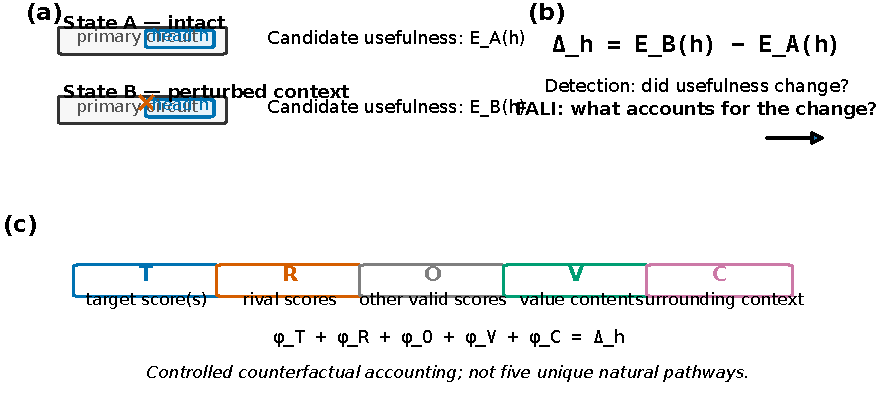
\includegraphics[width=\linewidth]{figures/Fig1.pdf}
  \caption{\textbf{FALI explains a conditional change rather than detecting it.}
  A selected attention head has output-grounded causal usefulness $E_A(h)$ in an intact context and $E_B(h)$ after a prespecified circuit perturbation.
  Their difference $\Delta_h$ is the conditional gain to be explained.
  FALI constructs controlled hybrid interventions over target scores ($T$), rival scores ($R$), other valid scores ($O$), value content ($V$), and surrounding-network context ($C$), and allocates the endpoint change among these factors.
  The method is hypothesis-driven: the candidate head and task-relevant target are specified before FALI analysis.}
  \label{fig:fali-overview}
\end{figure}

\begin{figure}[t]
  \centering
  % 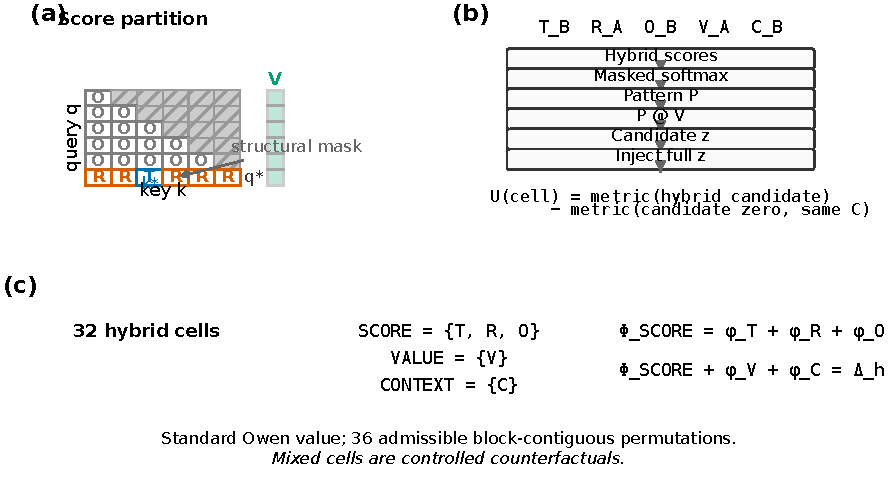
\includegraphics[width=\linewidth]{figures/Fig2.pdf}
  \caption{\textbf{FALI constructs an output-grounded 32-cell intervention game.}
  Structurally valid attention scores are partitioned into the task-target coordinate(s) $T$, rivals $R$ in the same query row, and all other valid scores $O$; $V$ denotes the candidate value tensor and $C$ the surrounding intact or perturbed computation.
  Each hybrid score tensor is passed through the model's masked softmax, combined with the selected values, and injected as the candidate's full head output.
  Utility is the task metric relative to a candidate-zero run in the same context.
  Standard Owen attribution under $\mathrm{SCORE}=\{T,R,O\}$, $\mathrm{VALUE}=\{V\}$, $\mathrm{CONTEXT}=\{C\}$ allocates interactions while reconciling the fine score attributions with the coarse three-factor game.}
  \label{fig:fali-game}
\end{figure}

\begin{figure}[t]
  \centering
  % 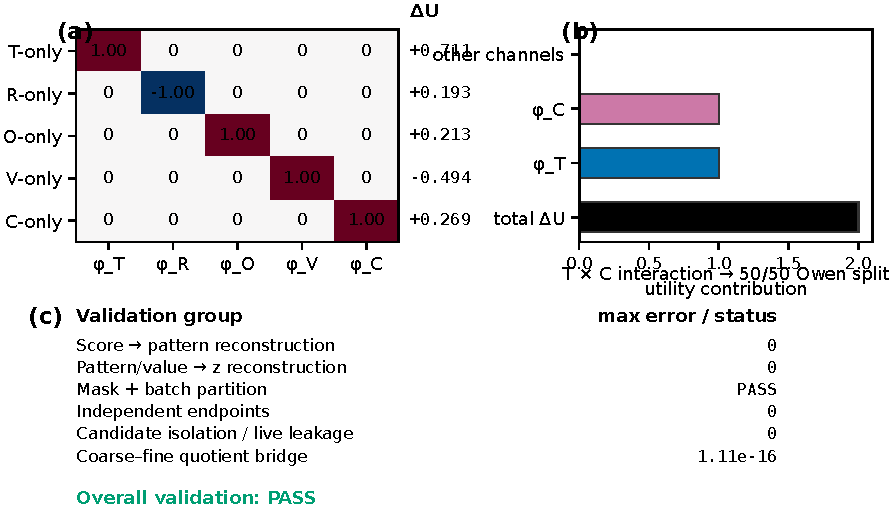
\includegraphics[width=\linewidth]{figures/Fig3.pdf}
  \caption{\textbf{FALI recovers controlled ground truth and satisfies implementation invariants.}
  (a) In five deterministic attention systems where only one of $T$, $R$, $O$, $V$, or $C$ differs between endpoints, the entire endpoint change is assigned to the manipulated factor up to floating-point error.
  Rows are normalized by their own absolute endpoint change for visual comparison; raw $\Delta U$ is annotated.
  (b) A constructed pure $T\times C$ interaction yields an equal Owen split between $T$ and $C$, as analytically expected.
  (c) A randomly initialized two-layer TransformerLens model independently validates score-to-pattern and pattern/value-to-output reconstruction, endpoint identity, batch-safe partitions, candidate-isolation, live-computation leakage checks, and coarse--fine quotient reconciliation.
  These are implementation/ground-truth tests, not evidence that FALI's hybrid factors are unique natural pathways.}
  \label{fig:validation}
\end{figure}

\begin{figure}[t]
  \centering
  % 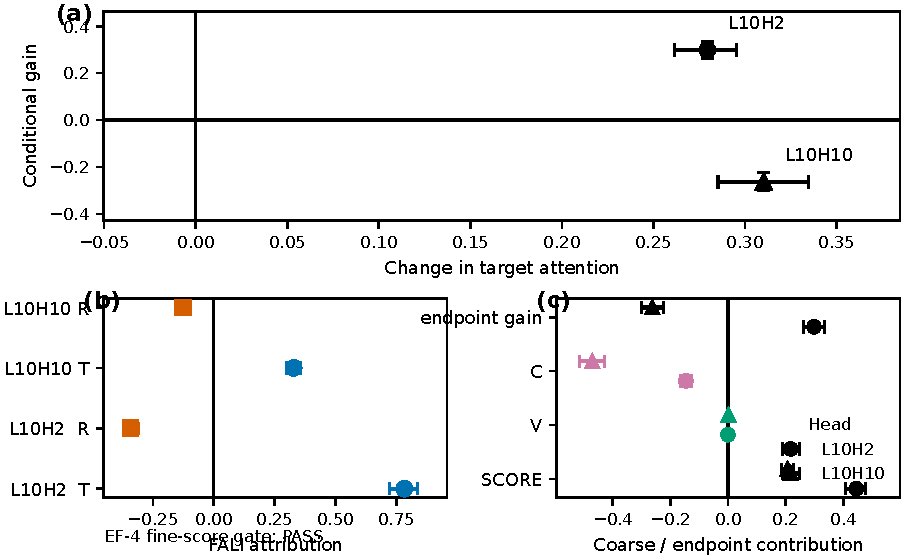
\includegraphics[width=\linewidth]{figures/Fig4.pdf}
  \caption{\textbf{Target-attention adaptation and positive functional recruitment are distinct in GPT-2 IOI.}
  (a) L10H2 and L10H10 both increase attention to the IO target after the canonical primary Name Movers are ablated, but their conditional gains have opposite signs: L10H2 becomes more causally useful whereas L10H10 becomes less useful on the broad canonical distribution.
  (b) Both heads nevertheless show positive target-score and negative rival-score FALI contributions; the preregistered EF-4 fine-score gate passes.
  (c) Coarse attribution clarifies the distinction: L10H10's positive SCORE contribution is outweighed by a substantially negative surrounding-context contribution, producing a negative endpoint change.
  Points are exact balanced means; intervals are hierarchical 95\% bootstrap CIs over the canonical template design.}
  \label{fig:gpt2-attention-recruitment}
\end{figure}

\begin{figure}[t]
  \centering
  % 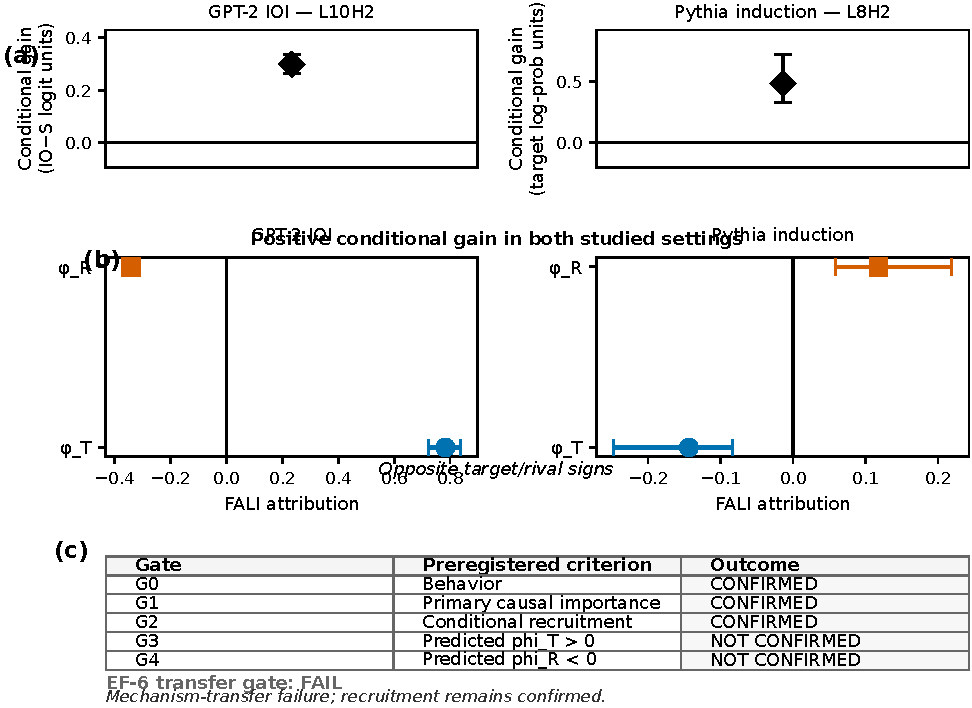
\includegraphics[width=\linewidth]{figures/Fig5.pdf}
  \caption{\textbf{Conditional recruitment occurs in both studied settings, but the preregistered fine-score mechanism reverses.}
  (a) GPT-2 IOI L10H2 and Pythia-160M induction L8H2 both have positive conditional gain after their respective primary interventions; axes are kept task-specific because the metrics use different units.
  (b) Their FALI target/rival decompositions have opposite signs: GPT-2 is target-positive/rival-negative, whereas Pythia is target-negative/rival-positive.
  (c) Accordingly, the preregistered Pythia transfer test confirms induction behavior, primary-head importance, and conditional recruitment (G0--G2) but fails both sign-transfer gates (G3--G4), so EF-6 is a failed mechanism-transfer hypothesis rather than a failed recruitment result.
  Intervals are the preregistered 95\% bootstrap CIs for each experiment.}
  \label{fig:cross-setting-reversal}
\end{figure}
